\section{Background} \label{sec:background}

% JOHANN -> TODO. I merged section 2 and 3 in this file.

% TODO - From reviewer 2 : Most of the background should be already known by readers and can be shortened/omitted. RESTful technologies are of daily use for anyone interested on Web Technologies.

% TODO - From reviewer 2 : Do not spend an entire section on someone's else work. You can introduce the maturity model as part of the background (even omitting the figure), provide appropriate references and discuss its disadvantages.
% Antoine -> I think we should keep the figure of the maturity model, it is a very good visual helper to its understanding.

This section describes the main concepts related to the design and implementation of Semantic Restful Web APIs and the process of selecting an API functionality.

% Antoine: to me, we can remove this subsection
%\subsection{REST}

%The REST architectural style imposes constraints on the design of a distributed system to guarantee the following properties: extensibility, evolution, loose-coupling and easy browsing~\cite{FieldingThesis}. To achieve this goal, it proposes six constraints: (i) \textit{client-server}, (ii) \textit{stateless}, (iii) \textit{cache}, (iv) \textit{uniform interface}, (v) \textit{layered system} and (vi) \textit{code-on-demand}. The latter is optional. The \textit{uniform interface} constraint is itself defined by four constraints: (i) \textit{unique identification of resources}, (ii) \textit{manipulation of resources through representations}, (iii) \textit{self-descriptive messages} and (iv) \textit{hypermedia as the engine of application state (HATEOAS)}.

% Antoine: to me, we can remove this subsection
%\subsection{Semantic Web and Linked Data}

%The Semantic Web~\cite{TheSemanticWeb} envisions the Web as an open platform, where information is machine processable and unstructured. This vision allows to create complex queries gathering information on the whole Web, which would otherwise be impossible.  It also allows global knowledge to grow quickly and easily because this global knowledge can be distributed among the different stakeholders. To achieve this goal, the Semantic Web community offers a unique and comprehensive set of technologies, including a data model, query language, framework, database, ontological languages, exchange formats and more.

%The principles of Linked Data are an extension of the Semantic Web. They advise using meaningful URIs to name things and including links to other resources to create an interconnected information structure. 

%With Linked Data, the Semantic Web is becoming closer to the uniform interface of REST systems since these principles are equivalent: namely (i) \textit{unique identification of resources}, (ii) \textit{manipulation of resources through representations} and (iii) \textit{hypermedia as the engine of application state (HATEOAS)}. 

% Antoine: to me, this section should stay. The subject is not well known. Scholar gives 91 results for "semantic rest" and 171 for "semantic restful".
\paragraph{Semantic RESTful services}
Combining REST with Semantic Web and Linked Data looks is a promising path since  it enables the description of APIs that can change without breaking client applications. These APIs advertise their available state transitions, therefore enabling automatic composition to create high level services \cite{alarcon2015rest}, on which intelligent software agents can automatically discover the suite of operations to realize complex workflows and even make any API compatible with voice assistants. This is achieved by semantically enriching the data and operations of REST systems with Semantic Web ontology technologies and by linking resources to other resources, making browsing easier.

% Antoine: to me, this section should stay in a shortened version because precision on the implementation, the types and guards are not used in the rest of the paper.
%\subsection{Resource Model}

%A resource model aims to model REST systems in which resources are the central element. A resource is any kind of named element, e.g. a photo, a spreadsheet or a table. It has representations, e.g. in the form of a JSON document or even a jpg image, and state transitions, which availability depends on the current state of the system. State transitions can be viewed as operations, either on the resource itself or on others. A common transition refers to a reading operation of another resource. This transition creates a link between the two resources. In the rest of this paper, operations on the resource itself are called operations while operations on other resources are called links.

%It is important to note that, the notion of resources cannot be mapped to the notion of class or entity in an object model. Indeed, the distinction between the notion of class and role does not necessarily exist in a resource-oriented approach. As an illustration, \emph{Users} is a different type of resource than \emph{User}.

%as opposed to classes in object-oriented modeling, a collection of resources of type T is another kind of resource than T. As an illustration, \emph{Users} is a different type of resource than \emph{User}.

%A resource type behavior may be described with a state machine, as presented in \cite{Schreier:2011:MRA:1967428.1967434}. If a resource's state change, the resource stays of the same type, even if the implementation represents different states with different classes. Each state may have some operations only available in the given state, and others available in every states. Operations have guards, computed from the values of the resource properties and the context, for example the currently connected user.

%Everything can be modeled as resources, including descriptions of operations that could then be used to generate actual HTTP operations at runtime. This way, the number of concepts is lowered and the model contain its own description, which leads to systems where the data and their descriptions can be accessed through a single mechanism.

\subsection{Selecting an API functionality level}\label{sec:maturityLevel}

The first step an architect faces when designing a Web API is to select the features to support.
Architects use a maturity model to help them decide on the supported features. In general, a maturity model is a scale that represents to what level a technology complies with a given architecture. To reach a level, a technology must meet each constraint of the previous levels and of the targeted level.
Currently, the most used maturity model in industry is the Richardson Maturity Model \cite{RichardsonMaturityModel}, which targets building REST APIs. However, we recommend using the WS3 maturity model \cite{7195633} as it extends the Richardson one, and SoHA \cite{SoHA}, with Semantic REST API-enabling constraints.

\paragraph{The WS3 maturity model}

In \cite{7195633}, authors describe the WS3 maturity model for classifying Semantic REST Web APIs. WS3 aims at promoting the adherence to REST architectural principles and the adoption of Semantic Web technology to improve the design, reuse, integration and documentation of Web APIs. It classifies APIs along three independent dimensions: \textit{design}, \textit{profile} and \textit{semantic}, as shown in Fig. \ref{WS3}.

\begin{figure}[ht]
  \caption{WS3 Maturity Model (from \cite{7195633})}
  \centering
  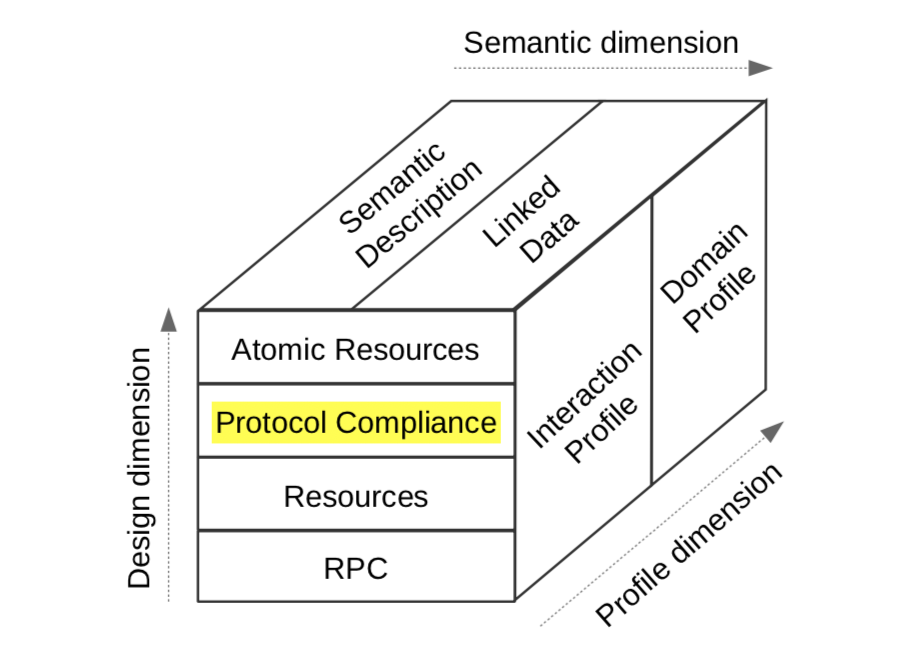
\includegraphics[width=0.47\textwidth]{figures/ws3-maturity-model.png}
  \label{WS3}
\end{figure}

The design dimension represents the different modeling strategies adopted for designing the technical access to a Web API through four levels. The first three levels are similar to the first three levels of the Richardson maturity model. The four levels are (i) RPC-like, (ii) resources have dedicated URI and the API is stateless, (iii) operations on a resource are mapped to HTTP verbs in compliance with the protocol and (iv) the smallest data unit that can be handled by operations is the resource.

The Profile dimension reflects the quality of documentation provided by the Web API through two levels. It takes into account only documentations that can be interpreted by software agents. The first level, interaction profile, requires the description of all available HTTP operations and how to trigger them. The second and final level, the domain profile, requires the description of domain specific details such as the order of operation execution, pre- and post-conditions, business constraints, etc. This level may be reached by providing hypermedia controls at runtime.

The Semantic dimension represents the use of semantic technologies through two levels. To reach the Semantic Description level, an API must semantically describe properties and operations of resources. Next level, Linked Data, is reach when the API semantically describes relationships between resources.

\paragraph{Usage}

In their paper, Salvadori \emph{et al.} propose to rate systems along each dimension independently, with a score going from 0 to n, n being the number of levels in the dimension.

For example, a non-documented API with no semantic support that reach level 3 of the Richardson Maturity Model will be rated D3-S0-P0. This means that the API reach the Protocol Compliance level of the Domain dimension and no level of both the Semantic and Profile dimensions.

%For another example, we consider building an API that supports HATEOAS and that provides a swagger-like documentation in the messages at runtime. HATEOAS is used to document available state transitions and to advertise users of the next operations to trigger in order to complete a given business process. This API is rated D3-S0-P2.

A system that supports HATEOAS and provides a swagger-like documentation along with the data, to inform the user of available state transitions, and of the operations to trigger to complete a given business process, is rated D3-S0-P2.

\paragraph{Discussion}

The WS3 maturity model is today the most complete maturity model to classify web semantic Rest API. Nevertheless, from our experience at XXX, we noticed two limitations to the applicability of the maturity model to a wider audience. These limitations are related to the Atomic Resources level and the abstraction chosen by the authors.

The Atomic resources constraint requires that the smallest data unit that can be handled by operations is the resource. Let us consider an API handling insurance contracts, that is readable and allows updating the postal address, email address and insurance manager, respecting the Atomic Resources constraint.  Two solutions can be considered. The first one is to create one resource, where every properties can be modified at once, which creates the risk that if two users want to modify two different information at the same time, only one may be made. With this solution, the API would have two operations. The second solution is to create four resources: one for the contract, one for the email address, one for the postal address and one for the manager. The API would have seven operations. The best trade-off would be to create one resource with four operations: (i) read, (ii) update email, (iii) update postal address and (iv) update manager. This solution lowers concurrency risks, the complexity for users and developers is in the middle of the two solutions offered by the Atomic Resources constraint and operations have a more meaningful name.

The second limitation relates to the granularity of the maturity levels. Indeed, each level implies more than one feature. This granularity allows for a coarse-grained categorization of systems. However, to precisely differentiate systems based on the features they implement, a deeper study is needed. Given two systems that reach P1, which means they describe all available HTTP operations and how to trigger them, one might also describe its authentication process and errors whereas the second does not. And yet they reach the same maturity level. As a second example, we consider two systems that describe HTTP operations and domain details such as the order of operations and the authentication process. One might support hypermedia controls whereas the other one has an OpenAPI documentation. These two features allow to reach the same maturity level: P2, even though they make a big difference from the client point of view.
